\documentclass[12pt]{beamer}
% \usetheme{umbc4}
\usetheme{moloch}

\usepackage{amsmath,amscd}
\usepackage{fontspec}
\usepackage{unicode-math}
\usepackage{pifont}
\usepackage{xcolor}
\usepackage[dvipsnames]{xcolor}

\definecolor{midgray}{rgb}{0.65, 0.65, 0.65}

% Set the slide body to black background with white text
\setbeamercolor{background canvas}{bg=black}
\setbeamercolor{normal text}{fg=white}

% Set the title bar to black background with white text
\setbeamercolor{frametitle}{bg=black, fg=white}

% Ensure other structural elements (bullets, etc.) are visible
\setbeamercolor{structure}{fg=white}

\setmainfont{Libertinus Serif}
\setsansfont{Libertinus Sans}
\setmathfont{STIX Two Math}

\newcommand{\FrameTitle}[2]{\frametitle{#1 \hfill \small\textnormal{\textcolor{midgray}{#2}}}}
\newcommand{\snl}{\vspace*{3pt}\\}
\newcommand{\nl}{\vspace*{1em}\\}
\newcommand{\vsp}{\vspace*{1em}}


\begin{document}
\title{\center{An Introduction to \\ Post-Quantum Cryptography \\}}
\author{\center{Manipal School of Information Sciences \\ Manipal \\}}
\date{\center{Friday, 24 April 2026}}
\maketitle

\begin{frame}\FrameTitle{Broad Outline}{Introduction}
    \begin{itemize}
        \item[\ding{52}] Classical Cryptography
        \item[--] Threats from Quantum Computing
        \item[--] Mitigating the Quantum Threats
        \item[\ding{52}] Post-Quantum Cryptography (PQC)
    \end{itemize}
    \vfill\normalsize\textit{\ding{52} involves hands-on Python programming}
\end{frame}

\begin{frame}\FrameTitle{The Plan}{Introduction}
    \begin{itemize}
        \item[\ding{52}] Classical Cryptography \hfill \textbf{\textasciitilde 2 hours}
        \item[--] Threats from Quantum Computing \hfill \textbf{\textasciitilde 20 minutes}
        \item[--] Mitigating the Quantum Threats \hfill \textbf{\textasciitilde 20 minutes}
        \item[\ding{52}] Post-Quantum Cryptography \hfill \textbf{\textasciitilde 1.5 hours}
    \end{itemize}
    \vfill\normalsize\textit{\ding{52} involves hands-on Python programming}
\end{frame}

\begin{frame}\FrameTitle{The Plan - Details}{Introduction}
    \begin{itemize}
        \item Classical Cryptography \hfill \textbf{\textasciitilde 2 hours}
        \begin{itemize}
            \item Primitives
            \item Protocols
            \item Computational Hardness Assumptions
        \end{itemize} \vsp
        \item Threats from Quantum Computing \hfill \textbf{\textasciitilde 20 minutes} \vsp
        \item Mitigating the Quantum Threats \hfill \textbf{\textasciitilde 20 minutes} \vsp
        \item Post-Quantum Cryptography \hfill \textbf{\textasciitilde 1.5 hours}
        \begin{itemize}
            \item Quantum-Resistant Computational Problems
            \item Principles of Lattice-Based Cryptography
            \item ML-KEM and ML-DSA schemes
        \end{itemize}
    \end{itemize}
\end{frame}


\begin{frame}\FrameTitle{A General Note}{Introduction}
    \large\textbf{Cryptography is fun because it is a blend of}
    \begin{itemize}
        \item[] \hspace*{2em} Mathematics
        \item[] \hspace*{2em} Computational Complexity Theory
        \item[] \hspace*{2em} Algorithms and Programming
        \item[] \hspace*{2em} Systems Security
    \end{itemize}
\end{frame}

\begin{frame}\FrameTitle{Want to Do  Cryptography?}{Introduction}
    \large\textbf{Science and engineering in equal parts}
    \begin{itemize}
        \item[] \hspace*{2em} Mathematics
        \item[] \hspace*{2em} Computational Complexity Theory
        \item[] \hspace*{2em} Algorithms and Programming
        \item[] \hspace*{2em} Systems Security
    \end{itemize}
\end{frame}

\begin{frame}\FrameTitle{A Useful Tip}{Introduction}
    {\center{\LARGE\textbf{Do not hesitate to ask questions!}}}
\end{frame}

\begin{frame}\FrameTitle{But Wait...}{Introduction}
    %\center{\Huge\textbf{\color{Apricot}{Why should I care?}}\\}
    \center{
\includegraphics[width=0.95\textwidth]{images/why-care.png}}
\end{frame}

\begin{frame}\FrameTitle{\color{Apricot}{Why Should I Care?}}{Introduction}
    {\Large{\text{Cryptography is pervasive}}}\nl

    \begin{itemize}
        \item[--] Aadhaar
        \item[--] UPI
        \item[--] TLS (\textit{and} HTTPS)
        \item[--] Signal/WhatsApp
        \item[--] GitHub (\textit{with} SSH authentication)
        \item[--] WireGuard (VPN support in Linux kernel)
        \item[--] Cryptocurrencies
        \item[...]
    \end{itemize}
\end{frame}

\begin{frame}\FrameTitle{Why Should I Care?}{Introduction}
    \large {It is believed that the \textit{quantum devices} of the future
            have the computational power to break cryptography schemes
            based on asymmetric/public key methods.}\nl
    \vspace*{1em}
    \large {Today, we will learn a few ideas that are meant to protect \textit{classical}
            cryptography from \textit{quantum adversaries}.}
\end{frame}

\begin{frame}\FrameTitle{Demystifying the Buzz}{Introduction}
    Classical Computers and Algorithms\nl
    \vspace*{0.5em}
    Quantum Computers and Quantum Algorithms\nl
    \vspace*{0.5em}
    Post-Quantum Cryptography (PQC)\vspace*{2pt}
    \begin{itemize}
        \item[--] It is \textbf{NOT post-quantum computing}
        \item[--] It is \textit{simply} post-quantum cryptography
        \item[--] You \textbf{\textit{don't}} need a quantum computer to do PQC!
    \end{itemize}
\end{frame}

\begin{frame}\FrameTitle{The Indian Context}{Introduction}
    {\Large{\textbf{PQC Readiness In the Works...}}}\nl

    NITI Aayog's Roadmap.\\
    {\color{Dandelion}{\texttt{niti\_roadmap\_quantum\_powered\_economy.pdf}}}\nl

    DST's Report\\
    {\color{Dandelion}{\texttt{dst\_quantum\_safe\_ecosystem.pdf}}}\nl

    Society for Electronic Transactions and Security.\\
    {\color{Dandelion}{\texttt{pki\_pqc\_india.pdf}}}\nl

    CERT-In and SISA Whitepaper.\\
    {\color{Dandelion}{\texttt{certin\_quantum\_readiness.pdf}}}\nl

    \vfill \textsuperscript{\textdagger}\scriptsize\texttt{PDF documents are available in the \textbf{ref} directory}
\end{frame}

\begin{frame}\FrameTitle{Getting Started...}{Introduction}
    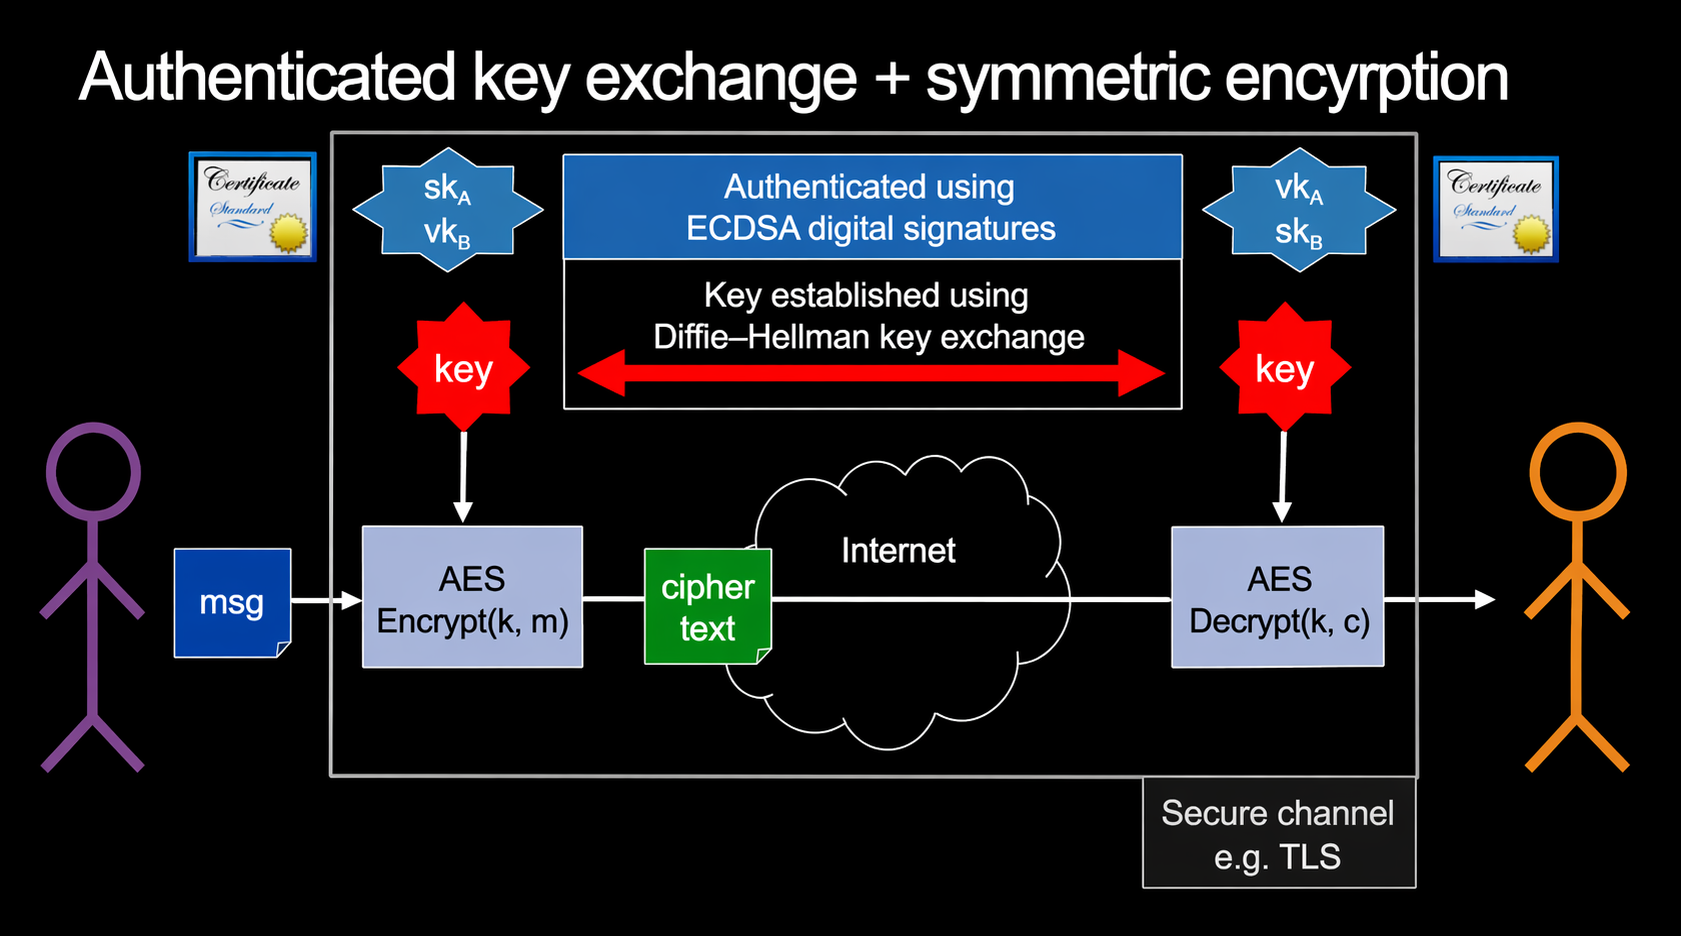
\includegraphics[width=0.9\textwidth]{images/generic-protocol.png}

    \vspace*{1em}
    {\large Don't worry if you don't understand all the terms!}
\end{frame}


\begin{frame}\FrameTitle{Basic Terms and Ideas}{Introduction}
    {\large\color{Apricot}{Primitives and Constructions}}\nl

    -- Primitives
    \begin{itemize}
        \item Pseudorandom Generators (PRGs)
        \item Hash functions
    \end{itemize}
    \vsp
    -- Constructions
    \begin{itemize}
        \item Key Derivation Functions (KDFs)
        \item Message Authentication Codes (MACs)
    \end{itemize}
\end{frame}

\begin{frame}\FrameTitle{Basic Terms and Ideas}{Introduction}
    {\large\color{Apricot}{Schemes and Protocols}}\nl

    -- Schemes
    \begin{itemize}
        \item Digital signatures
        \item Symmetric-key encryption methods
        \item Public-key encryption
    \end{itemize}
    \vsp
    -- Protocols
    \begin{itemize}
        \item Diffie-Hellman Key Exchange
        \item Transport Layer Security (TLS)
        \item Signal (\textit{and} Whatsapp) Messaging Protocol
    \end{itemize}
\end{frame}


\begin{frame}\FrameTitle{A Sample Protocol - TLS 1.3}{Introduction}
    \href{https://www.rfc-editor.org/rfc/rfc8446.html\#appendix-B.4}{Cipher Suites}\nl
    \href{https://www.rfc-editor.org/rfc/rfc8446.html\#appendix-B.3.1.3}{Signature Algorithms}\nl
    \href{https://www.rfc-editor.org/rfc/rfc8446.html\#section-7.4.2}{Diffie-Hellman}\nl
    \vspace*{1em}
    \href{https://www.rfc-editor.org/rfc/rfc8446.html\#page-93}{Key Schedule}\nl

\end{frame}

\begin{frame}\FrameTitle{}{Introduction}
    \vfill
    \center{\Huge{\textbf{Questions?}}}
    \vfill
    Next Session: \textbf{Hands-on Classical Cryptography}
\end{frame}

\end{document}